\documentclass{article} % For LaTeX2e
\usepackage{nips14submit_e,times}
\usepackage{hyperref}
\usepackage{url}
\usepackage{amsmath,amssymb}
\usepackage{booktabs,multirow}
\usepackage[backend=bibtex,
            style=numeric,
            firstinits=true,
            natbib=true]{biblatex}
\usepackage{graphicx}
\usepackage{subfig}
\bibliography{nips2014lin}


\title{A Variational Framework for Gaussian Models with Nonlinear Likelihoods}


\author{
David S.~Hippocampus\thanks{Use footnote for providing further information
about author (webpage, alternative address)---\emph{not} for acknowledging
funding agencies.} \\
Department of Computer Science\\
Cranberry-Lemon University\\
Pittsburgh, PA 15213 \\
\texttt{hippo@cs.cranberry-lemon.edu} \\
\And
Coauthor \\
Affiliation \\
Address \\
\texttt{email} \\
}

% The \author macro works with any number of authors. There are two commands
% used to separate the names and addresses of multiple authors: \And and \AND.
%
% Using \And between authors leaves it to \LaTeX{} to determine where to break
% the lines. Using \AND forces a linebreak at that point. So, if \LaTeX{}
% puts 3 of 4 authors names on the first line, and the last on the second
% line, try using \AND instead of \And before the third author name.

\newcommand{\fix}{\marginpar{FIX}}
\newcommand{\new}{\marginpar{NEW}}
%% Define bracket commands (normal, square and curly).
\newcommand{\brac} [1]  {\ensuremath{\left({#1}\right)}}
\newcommand{\sbrac}[1]  {\ensuremath{\left[{#1}\right]}}
\newcommand{\cbrac}[1]  {\ensuremath{\left\{{#1}\right\}}}
\newcommand{\abrac}[1]  {\ensuremath{\left\langle{#1}\right\rangle}}


%% Symbols

% General
\newcommand{\test}       {\ensuremath{^{*}}}
\newcommand{\testT}      {\ensuremath{^{*\top}\!}}
\newcommand{\ttest}      {\ensuremath{^{**}}}
\newcommand{\real}  [1] {\ensuremath{\mathbb{R}^{#1}}}
\newcommand{\ident} [1] {\ensuremath{\mathbf{I}_{#1}}}

% Variables
\newcommand{\lstate}    {\ensuremath{\mathbf{f}}}
\newcommand{\lcov}      {\ensuremath{\boldsymbol{\Sigma}}}
\newcommand{\obs}       {\ensuremath{\mathbf{y}}}
\newcommand{\hyper}     {\ensuremath{\boldsymbol{\theta}}}
\newcommand{\prmean}    {\ensuremath{\boldsymbol{\mu}}}
\newcommand{\prcov}     {\ensuremath{\mathbf{K}}}
\newcommand{\pomean}    {\ensuremath{\mathbf{m}}}
\newcommand{\pocov}     {\ensuremath{\mathbf{C}}}
\newcommand{\xcov}      {\ensuremath{\boldsymbol\Sigma_{\obs\pomean}}}
\newcommand{\Sobs}      {\ensuremath{\mathcal{Y}}}
\newcommand{\Sfunc}     {\ensuremath{\mathcal{M}}}
\newcommand{\scoef}     {\ensuremath{\kappa}}
\newcommand{\Sw}        {\ensuremath{w}}
\newcommand{\Kgain}     {\ensuremath{\mathbf{H}}}
\newcommand{\Linmat}    {\ensuremath{\mathbf{A}}}
\newcommand{\intcpt}    {\ensuremath{\mathbf{b}}}
\newcommand{\Fengy}     {\ensuremath{\mathcal{F}}}
\newcommand{\step}      {\ensuremath{\alpha}}
\newcommand{\jacob}[1]  {\ensuremath{\mathbf{J}_{#1}}}

% Augmented systems
\newcommand{\augobs}    {\ensuremath{\mathbf{z}}}
\newcommand{\augcov}    {\ensuremath{\mathbf{S}}}
\newcommand{\augLinmat} {\ensuremath{\mathbf{B}}}
\newcommand{\augintcpt} {\ensuremath{\mathbf{c}}}

% Gaussian Process
\newcommand{\obss}      {\ensuremath{y}}
\newcommand{\lstates}   {\ensuremath{f}}
\newcommand{\Lins}      {\ensuremath{a}}
\newcommand{\Linvec}    {\ensuremath{\mathbf{a}}}
\newcommand{\intcpts}   {\ensuremath{b}}
\newcommand{\inobs}     {\ensuremath{\mathbf{x}}}
\newcommand{\kernl}     {\ensuremath{k}}
\newcommand{\Kernl}     {\ensuremath{\mathbf{k}}}
\newcommand{\KERNL}     {\ensuremath{\mathbf{K}}}
\newcommand{\lvar}      {\ensuremath{\sigma^2}}
\newcommand{\lstd}      {\ensuremath{\sigma}}
\newcommand{\Lvar}      {\ensuremath{\boldsymbol\Lambda}}
\newcommand{\pomeans}   {\ensuremath{m}}
\newcommand{\pocovs}    {\ensuremath{C}}
\newcommand{\xcovs}     {\ensuremath{\Sigma}}
\newcommand{\khyper}    {\ensuremath{\theta}}
\newcommand{\khypers}   {\ensuremath{\boldsymbol\theta}}


%% Operations
\newcommand{\transpose}  {\ensuremath{^{\!\top}}}
\newcommand{\inv}        {\ensuremath{^{\text{-}1}}}
\newcommand{\deter}[1]   {\ensuremath{\left|{#1}\right|}}
\newcommand{\trace}[1]   {\ensuremath{\text{tr}\!\brac{#1}}}
\newcommand{\diag}[1]    {\ensuremath{\text{diag}\!\brac{#1}}}
\newcommand{\expec}[2]   {\ensuremath{\abrac{#2}_{#1}}}
\newcommand{\expece}[2]  {\ensuremath{\mathbb{E}_{#1}\!\sbrac{#2}}}
\newcommand{\evar} [2]   {\ensuremath{\mathbb{V}_{#1}\!\sbrac{#2}}}
\newcommand{\KL}[2]      {\ensuremath{\text{KL}\!\sbrac{{#1}\!\parallel\!{#2}}}}
\newcommand{\entropy}[1] {\ensuremath{\mathbb{H}\sbrac{#1}}}
\newcommand{\lnorm}[2]   {\ensuremath{\left\|{#2}\right\|_{{#1}}}}


%% Functions, PDFs etc
\newcommand{\nonlin}[1] {\ensuremath{g\!\brac{{#1}}}}
\newcommand{\augnonlin}[1] {\ensuremath{h\!\brac{{#1}}}}
\newcommand{\prob}  [1] {\ensuremath{p\!\brac{#1}}}
\newcommand{\probC} [2] {\ensuremath{p\!\left({#1}\middle\vert{#2}\right)}}
\newcommand{\qrob}  [1] {\ensuremath{q\!\brac{#1}}}
\newcommand{\qrobC} [2] {\ensuremath{q\!\left({#1}\middle\vert{#2}\right)}}
\newcommand{\gaus}  [1] {\ensuremath{\mathcal{N}\!\brac{#1}}}
\newcommand{\gausC} [2] {\ensuremath{\mathcal{N}\!\left({#1}\middle\vert{#2}\right)}}
\newcommand{\bern}  [1] {\ensuremath{\textrm{Bern}\!\brac{#1}}}
\newcommand{\bernC} [2] {\ensuremath{\textrm{Bern}\!\left({#1}\middle\vert{#2}\right)}}
\newcommand{\kfunc} [2] {\ensuremath{\kernl\!\brac{{#1}, {#2}}}}
\newcommand{\expon} [2] {\ensuremath{{#1}\!\times\!10^{#2}}}


%% Operators
\DeclareMathOperator*{\argmax}{\operatorname*{argmax}}
\DeclareMathOperator*{\argmin}{\operatorname*{argmin}}


%\nipsfinalcopy % Uncomment for camera-ready version

\begin{document}


\maketitle

\begin{abstract}
\end{abstract}

\section{Introduction}

\section{Linearised Gaussian Models}

\section{Linearised Gaussian Processes}

\section{Experiments}


\subsection{Various Nonlinear Functions}

\begin{figure}[htb]
    \subfloat[][$\nonlin{\lstate} = 2\text{sign}\!\brac{\lstate} + \lstate^3$]
        {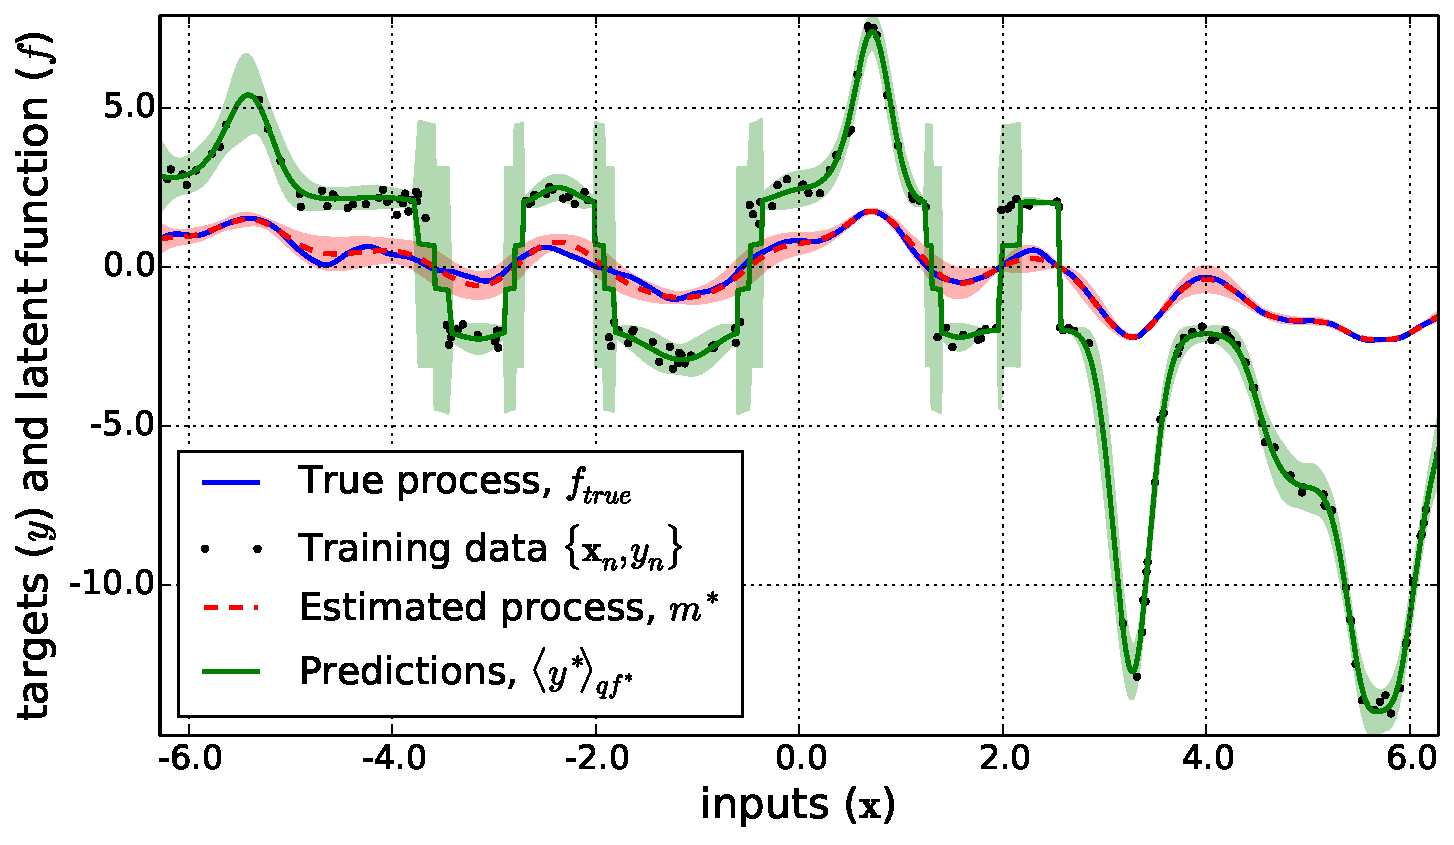
\includegraphics[width=0.5\linewidth]{fig/signdemo}\label{sub:sign}}
    \subfloat[][$\nonlin{\lstate} = \lfloor 5\lstate \rceil$]
        {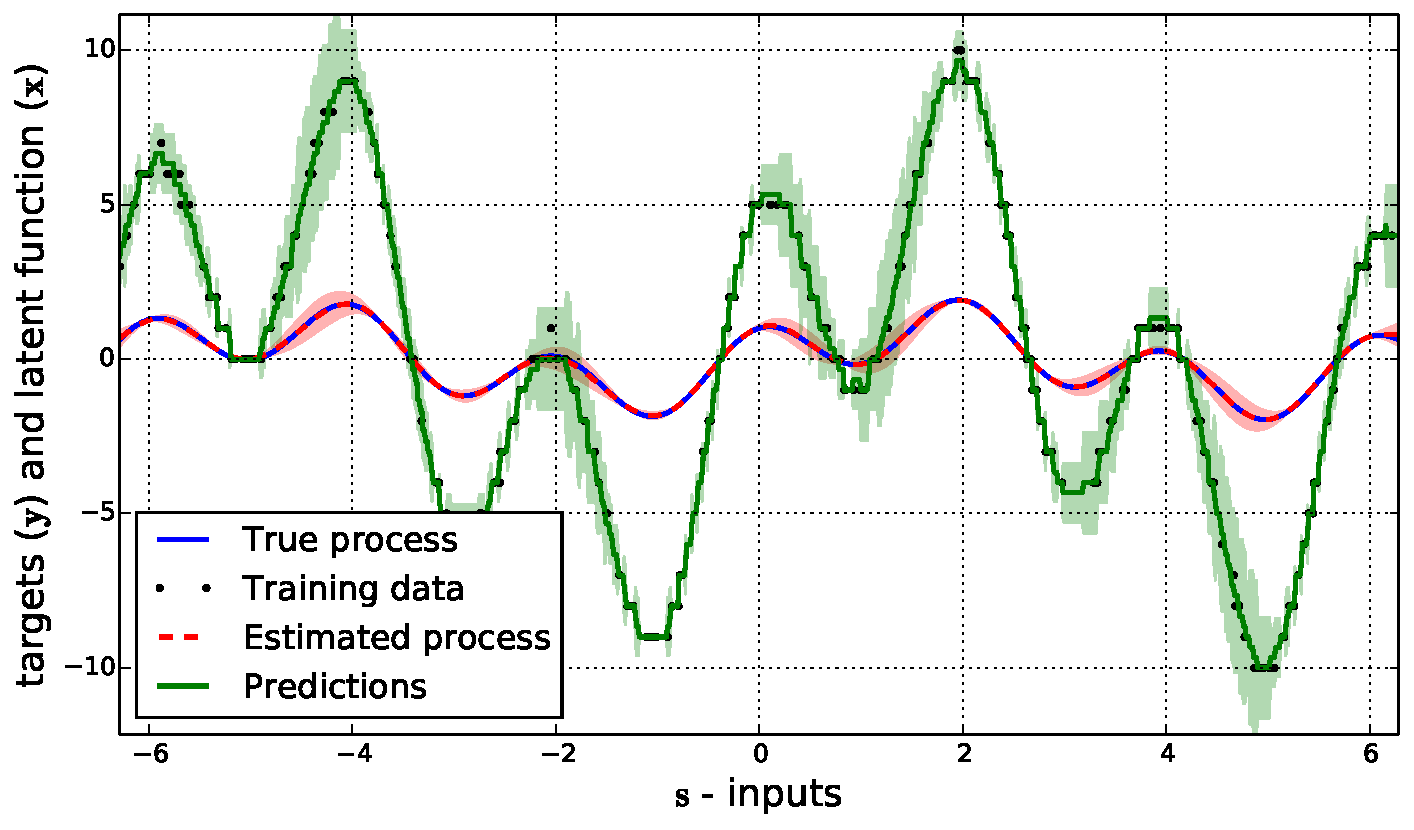
\includegraphics[width=0.5\linewidth]{fig/rounddemo}\label{sub:rnd}}\\
    \subfloat[][MAP trace -- poor hyperparameter values]
        {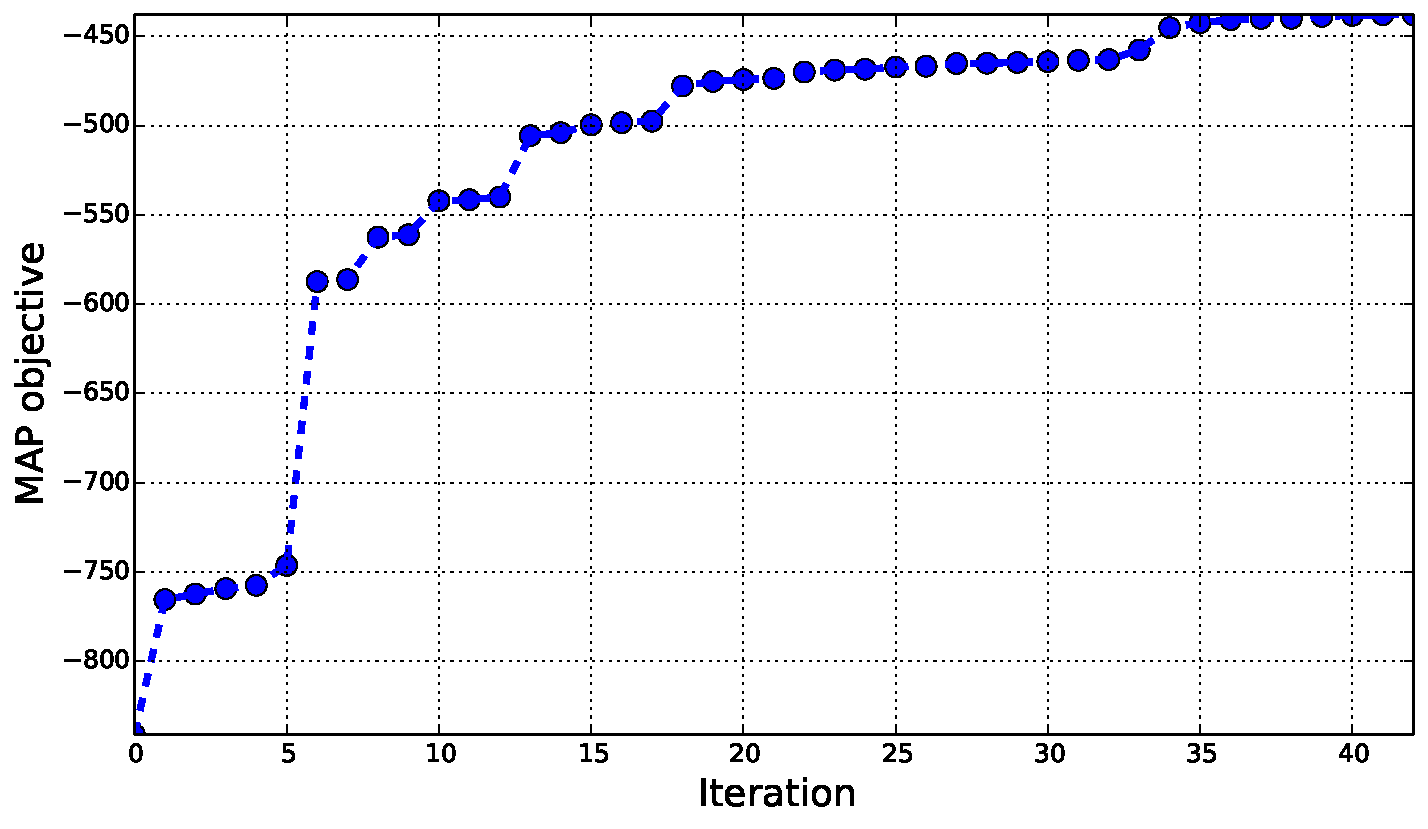
\includegraphics[width=0.5\linewidth]{fig/trace_beg}\label{sub:mapb}}
    \subfloat[][MAP trace -- near optimal hyperprameter values]
        {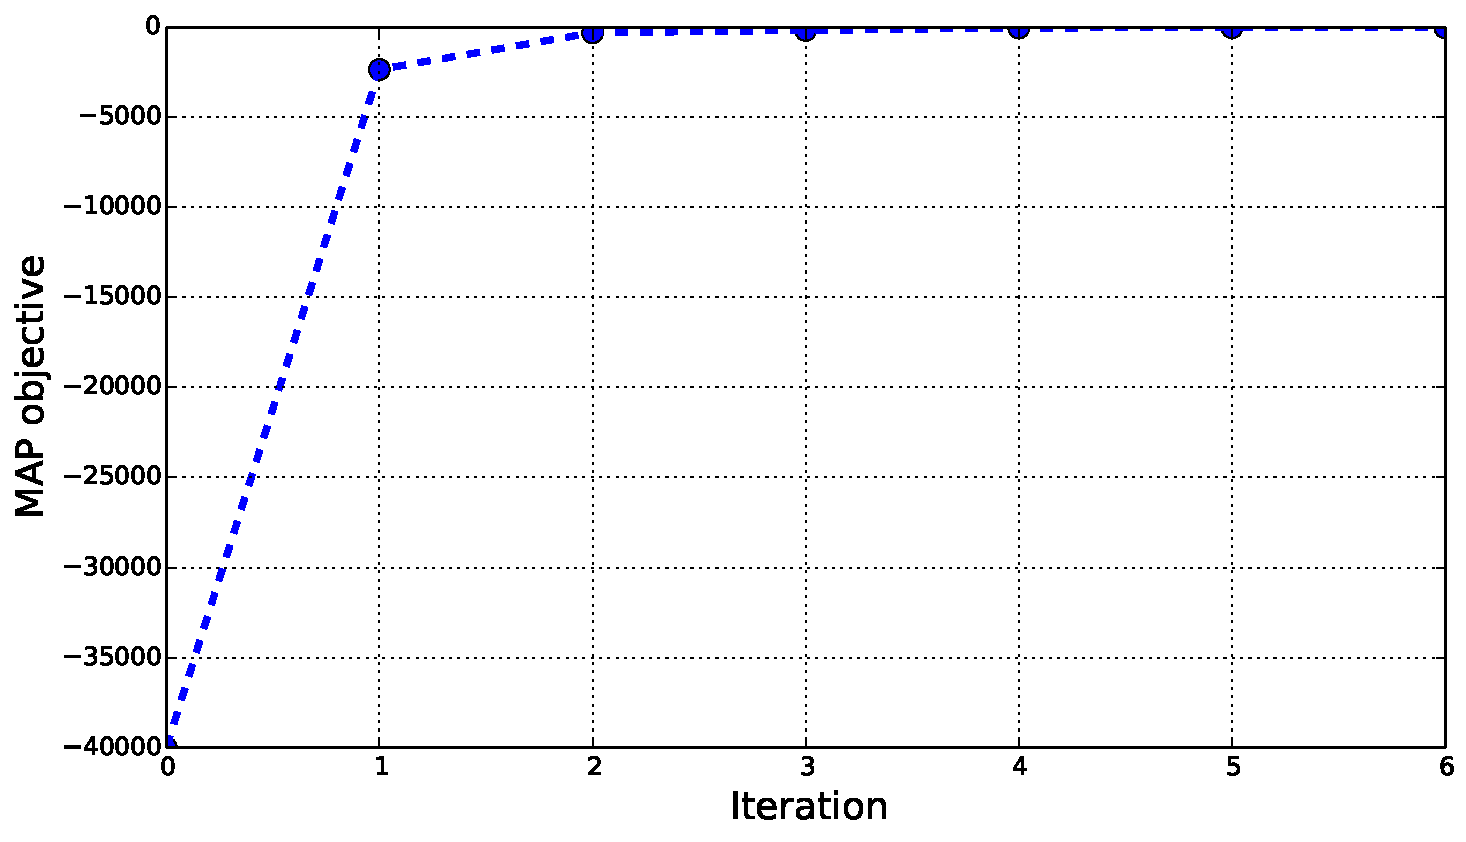
\includegraphics[width=0.5\linewidth]{fig/trace_end}\label{sub:mape}}
    \caption[]{Example of learning the statistically linearised GP with
        non-differentiable nonlinear functions in \subref{sub:sign} and
        \subref{sub:rnd}. Typical traces from the MAP objective function used
        to learn $\pomean$, \subref{sub:mapb} is from near the outset of
        learning the hyperparameters, and \subref{sub:mape} is near model
        convergence -- both terminated because of `divergence'.}
    \label{fig:learnex}
\end{figure}

\begin{table}[htb]
    \centering
    \small
    \caption[]{Results from running nonlinear likelihood GPs with various
        differentiable nonlinear functions. The true latent function is
        $\lstate_{\text{true}}\!\brac{\inobs} = \sin\!\brac{\inobs} 
            + \cos\!\brac{\pi\inobs}$.}
    \begin{tabular}{r|c| c c c c c c}
        \multirow{2}{*}{$\nonlin{\lstate}$} & \multirow{2}{*}{Algorithm} & 
            \multicolumn{2}{c}{$-\frac{1}{N\test}
                \log\probC{\lstates\test}{\obs,\lstate}$} &
            \multicolumn{2}{c}{SMSE $\lstates\test$ (\expon{}{-4})} &
            \multicolumn{2}{c}{SMSE $\obss\test$ (\expon{}{-4})} \\
        & & mean & std. & mean & std. & mean & std.\\
        \toprule
        $\lstate$ 
            & Statistical & $-$1.4453 & 0.0601 & 36.471 & 7.309 & -- & -- \\
            & Taylor & 14.2072 & 2.7953 & 54.674 & 8.890 & -- & -- \\
            & \cite{Opper2009} \\
            & Linear & $-$1.2793 & 0.0162 & 40.210 & 7.012 & -- & -- \\
        \midrule
        $\lstate^3 + \lstate^2 + \lstate$ 
            & Statistical & $-$2.1402 & 0.0604 & 27.725 & 6.097 & 36.239 
                & 5.089 \\
            & Taylor & 10.1842 & 1.9443 & 31.094 & 9.193 & 36.991 & 5.869 \\
            & \cite{Opper2009} \\
        \midrule
        $\exp\!\brac{\lstate}$ 
            & Statistical & $-$1.3858 & 0.2320 & 99.405 & 75.756 & 170.07 
                & 27.490 \\
            & Taylor & 15.1875 & 4.0084 & 235.10 & 82.551 & 174.70 & 26.181 \\
            & \cite{Opper2009} \\
        \midrule
        $\sin\!\brac{\lstate}$ 
            & Statistical & $-$0.8892 & 0.1259 & 152.75 & 32.744 & 858.63
                & 104.26 \\
            & Taylor & 20.1577 & 5.9408 & 387.67 & 131.13 & 889.80 & 127.22 \\
            & \cite{Opper2009} \\
        \midrule
        $\tanh\brac{2\lstate}$
            & Statistical & $-$0.5903 & 0.1132 & 395.96 & 40.270 & 602.24 
                & 60.622 \\
            & Taylor & 23.7728 & 8.9093 & 894.32 & 523.64 & 606.16 & 64.206 \\
            & \cite{Opper2009} \\
        \bottomrule
    \end{tabular}
\end{table}


\subsection{Binary Handwritten Digit Classification}

\begin{table}[htb]
    \centering
    \small
    \caption[]{Binary Gaussian process classifier performance on the USPS
        handwritten-digits dataset for numbers `3' and `5'.}
    \begin{tabular}{r| c c c c}
        Algorithm & Av.\ neg.\ ll. & Error rate (\%) 
            & $\log\brac{\sigma}$ & $\log\brac{l}$ \\
        \toprule
        GP -- Laplace & 0.11528 & 2.9754 & 2.5855 & 2.5823 \\
        GP -- EP & 0.07522 & 2.4580 & 5.2209 & 2.5315 \\
        SVM (RBF) & 0.07342 & 2.3286 & -- & -- \\
        Logistic Reg. & 0.11995 & 3.6223 & -- & -- \\
        \midrule
        GP -- Statistical & 0.11748 & 2.9754 &  2.8177 & 2.5504 \\
        GP --Taylor & 0.69293 & 42.4321 & 3.1268 & $-$0.1696 \\
        \bottomrule
    \end{tabular}
\end{table}

\section{Conclusion}

\subsubsection*{Acknowledgments}

\subsubsection*{References}
\printbibliography

\end{document}
